% Created 2020-10-09 Fri 19:08
% Intended LaTeX compiler: pdflatex
\documentclass[11pt]{article}
\usepackage[utf8]{inputenc}
\usepackage[T1]{fontenc}
\usepackage{graphicx}
\usepackage{grffile}
\usepackage{longtable}
\usepackage{wrapfig}
\usepackage{rotating}
\usepackage[normalem]{ulem}
\usepackage{amsmath}
\usepackage{textcomp}
\usepackage{amssymb}
\usepackage{capt-of}
\usepackage{hyperref}
\usepackage {indentfirst}
\usepackage [brazilian]{babel}
\usepackage [a4, top = 3cm, bottom = 2cm, inner = 3cm, outter = 3cm] {geometry}
\setlength {\parindent} {3em} \hypersetup{draft}
\addto\captionsbrazilian{\renewcommand{\figurename}{Fig.}}
\author{Alkindar Rodrigues, Anna Julia Lima}
\date{07 de Outubro de 2019}
\title{Relatório: Remoodle\\\medskip
\large Uma reimplementação de interfaces do Moodle IFSP}
\hypersetup{
 pdfauthor={Alkindar Rodrigues, Anna Julia Lima},
 pdftitle={Relatório: Remoodle},
 pdfkeywords={},
 pdfsubject={},
 pdfcreator={Emacs 27.1 (Org mode 9.3)}, 
 pdflang={English}}
\begin{document}

\maketitle

\section*{O Moodle}
\label{sec:org8121ad0}
Neste período de pandemia, quando as universidades tiveram que se
adaptar ao ensino a distância, o Moodle se tornou uma das ferramentas
usadas para tal, ganhando ainda mais importância em comparação ao que
tinha antes de março de 2020.
Esta plataforma de gestão de aprendizagem, segundo consta em seu
portal, promete auxiliar o ensino em diversas instituições provendo
``um sistema único, robusto, seguro e integrado''\footnote{Esta informação pode ser conferida na documentação da
plataforma, \href{https://docs.moodle.org/39/en/About\_Moodle\#Highly\_flexible\_and\_fully\_customisable}{disponivel aqui}, acessado em 07 de outrubro de 2020.}, mas que ao mesmo
tempo é altamente flexível, tanto em suas funcionalidades quanto em
sua interface.

Para tanto, as versões do sistema Moodle são colocadas em produção
a pedido dos próprios gestores das instituições que o utilizam, sendo
cada instância livre das demais quanto as funções e interfaces
que decide implementar.
Para além destas variações de instância a instância, diversas opções
de \emph{layout} são disponibilizadas para os usuários, e principalmente
educadores, que recebem opções \emph{drag and drop} para construir os
espaços de disciplinas, atividades, material de estudo e áreas de
entrega de tarefas.

Desta forma, tendo em vista o papel crescente das plataformas virtuais
de ensino, escolhemos para este trabalho a reelaboração de algumas
interfaces do Moodle IFSP.
As sessões que se seguem apresentarão uma análise acerca de algumas
interfaces altualmente em uso e alguns comentários de estudantes que
usam esta plataforma para manter a rotina de estudos em isolamento
social.
Posteriormente, serão apresentadas algumas propostas de refatoração
destas interfaces, tendo em vista a sua usabilidade e guiadas pelos
comentários coletados dos usuários.

\subsection*{A interface do Moodle IFSP}
\label{sec:org444ffb6}
No escopo deste projeto, escolhemos três interfaces do portal Moodle
IFSP para reimplementar: a página inicial, aberta após o login na
plataforma, a página de disciplina, relativa a cada um dos cursos em
que o aluno está matriculado e a página de entrega de tarefas.  Estas
três interfaces foram escolhidas pois forma um caso de uso bastante
comum: a entrega de uma atividade por um estudante.

\subsubsection*{O painel de cursos}
\label{sec:org7c773eb}
A interface principal do Moodle IFSP, como vista nas fuguras
\ref{fig:org20b483b} e \ref{fig:org4a1469f}, está codificada nas cores da instuição (verde e branco)
e presenta 5 grandes áreas:
\begin{itemize}
\item Uma barra de navegação, no topo, com alguns menus \emph{drop-down} com
\emph{links} pra os diversos tipos de usuários, uma caixa de pesquisa,
alertas de notificações, \emph{chat}, email e outro menu \emph{drop-down} com
\emph{links} para acesso rápido às informações do usuário.
\item Uma barra lateral à esquerda, acessível por um botão na barra de
navegação, composta por botões para a página inicial, calendário
acadêmico, arquivos privados e um menu \emph{drop-down} com as
disciplinas em que o aluno está inscrito.
\item Uma área central, intitulada ``Resumo dos cursos'', com \emph{cards}
relativos a cada uma das disciplinas do aluno, seguida de outra área
(fora do \emph{print}) de cursos acessados recentemente, com os \emph{cards} semelhantes.
\item Uma barra lateral, cujo conteúdo completo não coube no \emph{print},
intitulada ``Linha do tempo'', com as entregas de tarefas, opções de
personalização desta (atrasadas, futuras, período de listagem),
seguida de:
\begin{itemize}
\item opções de acessiblidade;
\item usuários online;
\item calendário;
\item uma segunda lista chamada ``Próximos eventos'', com as avaliações
e tarefas futuras, e;
\item arquivos privados do usuário.
\end{itemize}
\item Um rodapé verde, com informações sobre os responsáveis sobre a
página e a localização do IFSP São Paulo.
\end{itemize}

Nota-se imediatamente alguns problemas com \emph{layout}: a repetição de
informações nesta tela, com a duplicação, das informações de
cursos atuais e tarefas futuras. Um botão para personalizar a página
flutua à direita, acima da barra lateral. A barra lateral à direita é
desproporcionalmente grande em relação aos demais elementos da página.

\subsubsection*{A página de disciplina}
\label{sec:org5ecd2c6}
Dentre as interfaces do portal Moodle, esta é uma das mais flexíveis
com relação ao \emph{layout}.  As figuras \ref{fig:org175281c}, \ref{fig:org12b39f8} e
\ref{fig:org86fdd05} apresentam \emph{prints} parciais de páginas de disciplinas
ofertadas no segundo semestre de 2020, enfocando a disposição das
aulas em cada uma. Consideramos estes \emph{prints} são ilustrativos acerca
da enorme flexiblidade em esta interface apresenta:

Vemos na figura \ref{fig:org175281c} uma árvore de tópicos. No primeiro nível
dela, cada elemento diz respeito a uma aula, com seu número e tópico
em texto grande.  Um nivel abaixo, vários \emph{links} com símbolo de
arquivos em pdf, contendo os materiais de aula.  Alguns elementos
deste nível, referentes a exercícios a serem entregues, possuem
subtópicos, com \emph{links} que levam à pagina de entrega de tarefas.  Os
tópicos no primeiro nível separados por uma linha horizontal, que
delimita o espaço de cada aula.

Um segundo \emph{layout} aplicado a esta página esta apresentado na imagem
\ref{fig:org12b39f8} neste, alguns \emph{links} foram disponiblizados no topo da
página, com um acesso a espaços de avisos e retirada de dúvidas, aulas
síncronas gravadas e uma calculadora online. Logo abaixo destes \emph{links},
vários blocos azuis se sobrepões, em um esquema de \emph{tabs} que expandem
o conteudo de uma aula abaixo (fora do \emph{print}). Estas podem ter um
tamanho qualquer, incluir videos, documentos pdf, word ou outros. Como
o espaço ocupado pelas \emph{tabs} é consideravelmente maior que a largura
da página, a linha é quebrada, descaracterizando uma barra de \emph{tabs}.

Por fim, o /layout/apresentado na \ref{fig:org86fdd05} é semelhante ao da figura
\ref{fig:org175281c}: é apresentada uma lista de caixas, com um título em letras
grandes e azuis, indicando um \emph{links}. No canto direito inferior das
caixas há alguns rótulos, indicando os materiais associados à aula:
documentos, tarefas, \emph{links} externos, e indicadores de progresso,
para tarefas com mais de uma etapa.

\subsubsection*{A página de entrega de tarefas}
\label{sec:org0f26a70}

\subsection*{Comentários de usuários sobre a inferface do Moodle IFSP}
\label{sec:orgd2ab9b2}


\section*{Propstas de refatoração}
\label{sec:orgea95203}

\section*{Wireframes}
\label{sec:org7c050d5}

\section*{Conclusão}
\label{sec:org2cb91c4}


\section*{Apêndice\hfill{}\textsc{ignore}}
\label{sec:org37e17ab}
\begin{figure}[htbp]
\centering
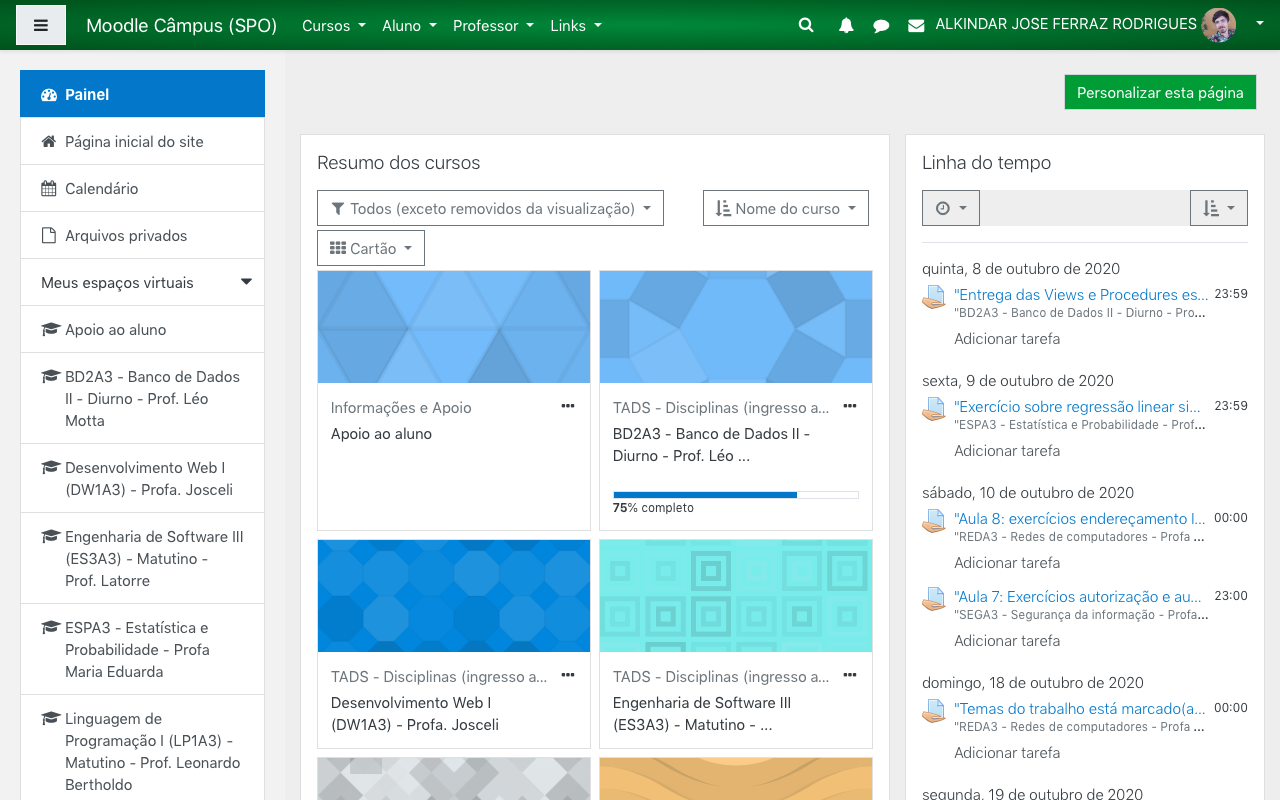
\includegraphics[width=.9\linewidth]{./media/painel.png}
\caption{\label{fig:org20b483b}Painel de cursos do Moodle IFSP}
\end{figure}
\begin{figure}[htbp]
\centering
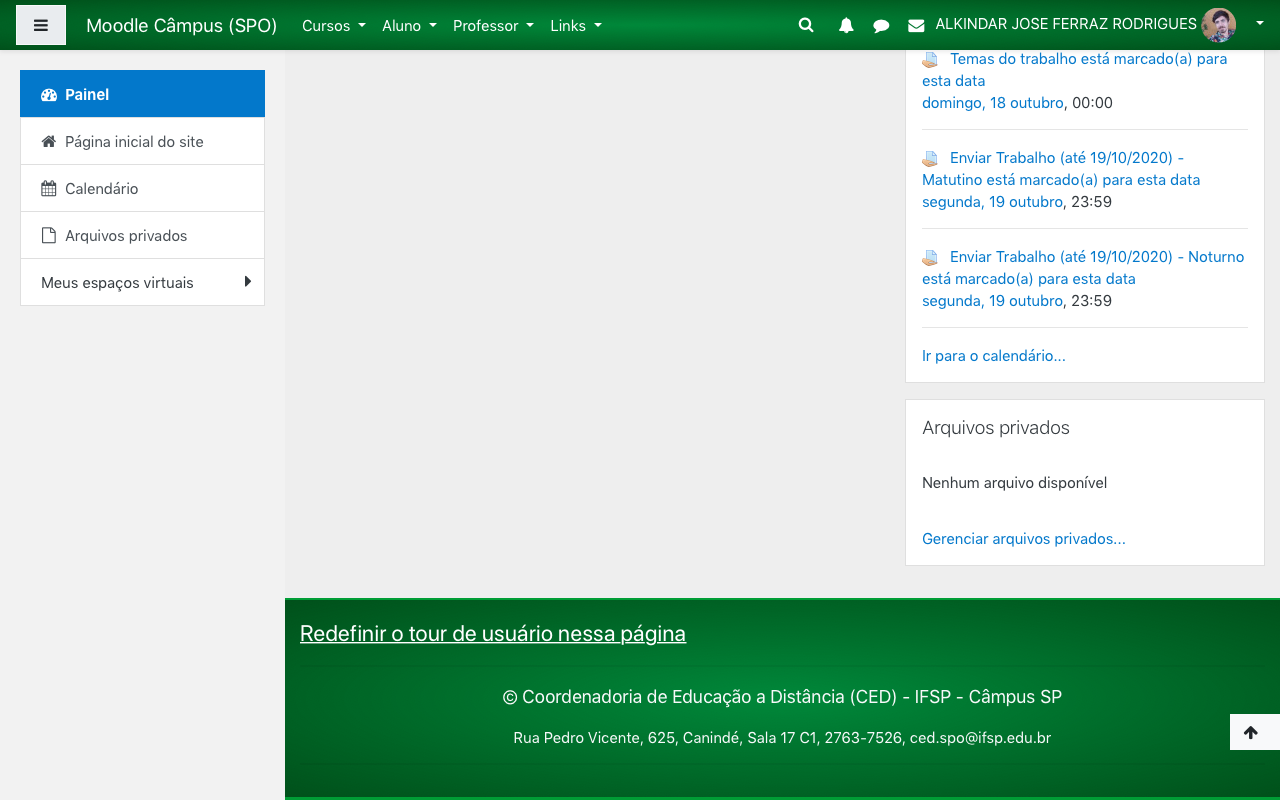
\includegraphics[width=.9\linewidth]{./media/painel_fim.png}
\caption{\label{fig:org4a1469f}Fim da página de painel de cursos do Moodle IFSP}
\end{figure}
\begin{figure}[htbp]
\centering
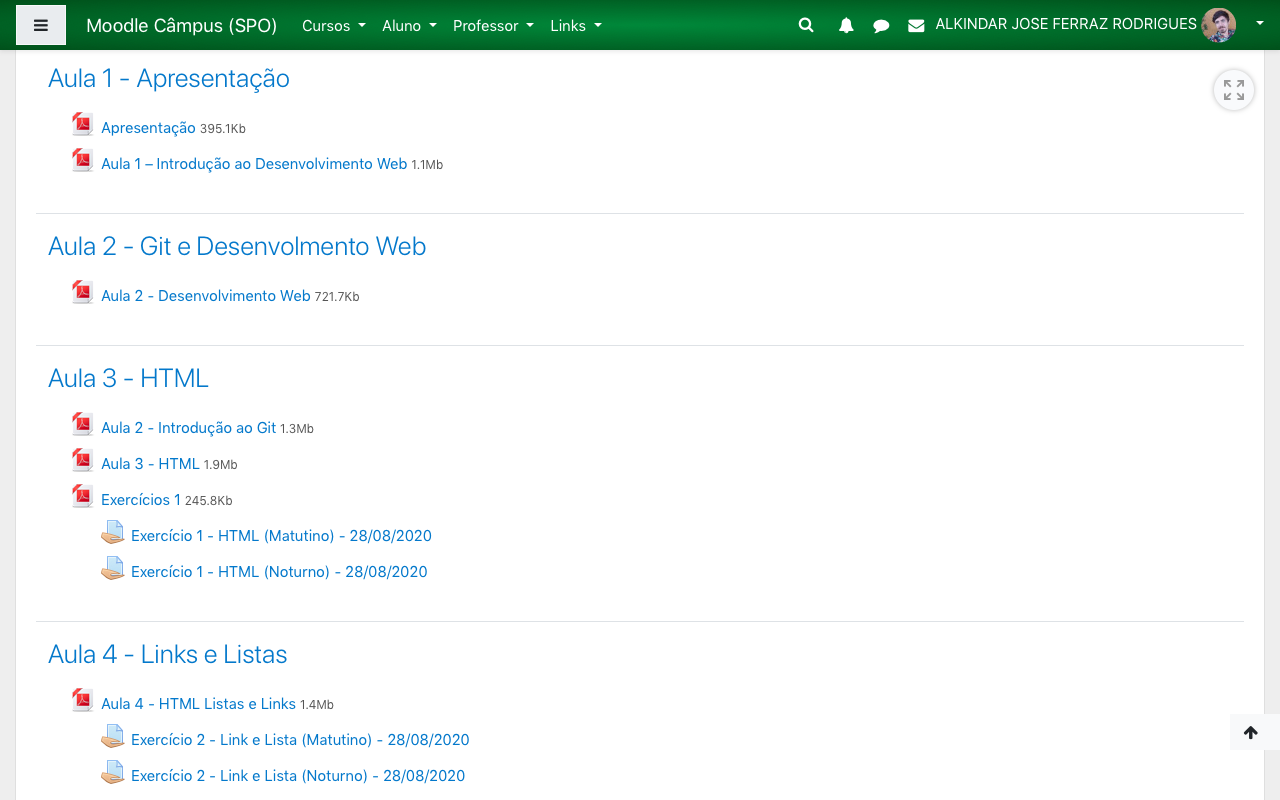
\includegraphics[width=.9\linewidth]{./media/disc_1.png}
\caption[\emph{Layout}]{\label{fig:org175281c}\emph{Layout} da página de disciplina: aulas e arquivos.}
\end{figure}
\begin{figure}[htbp]
\centering
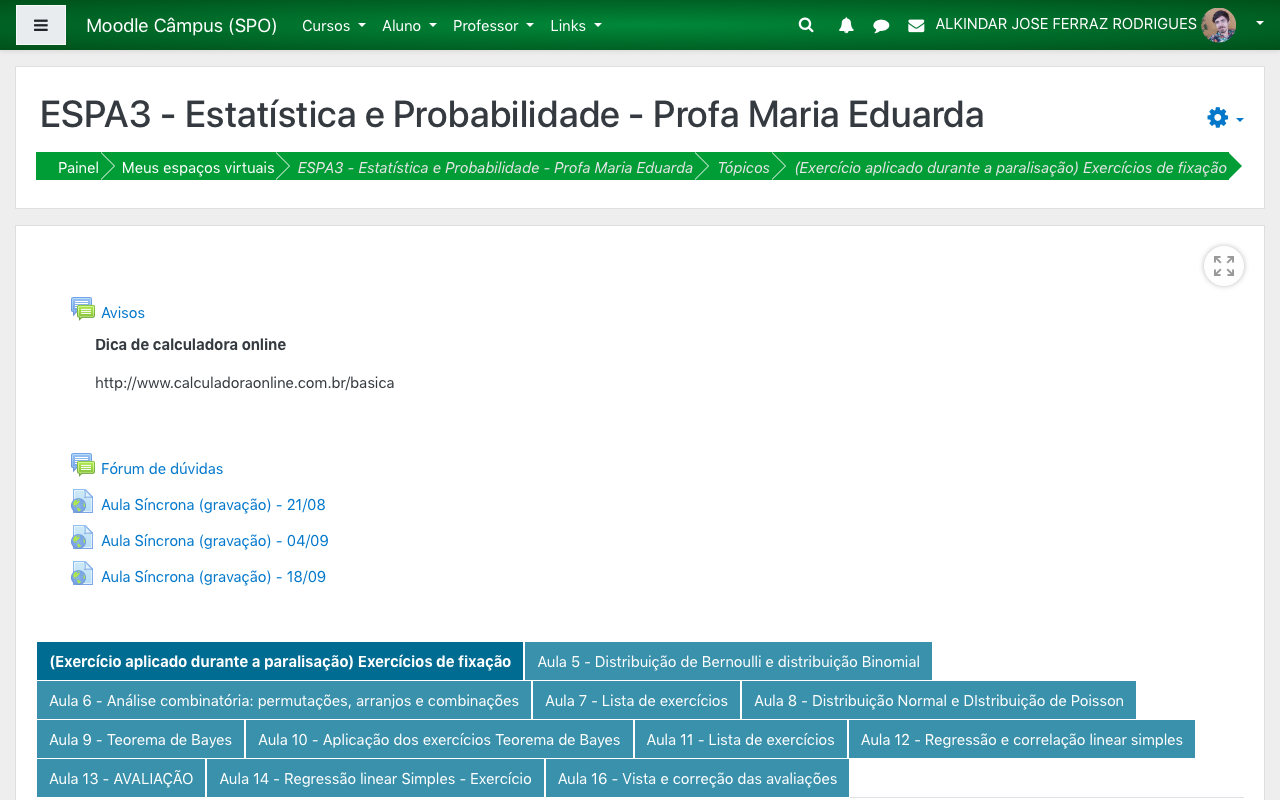
\includegraphics[width=.9\linewidth]{./media/disc_2.png}
\caption[\emph{tab}]{\label{fig:org12b39f8}\emph{Layout} da página de disciplina: tópicos em \emph{tab} que expandem o conteúdo da aula.}
\end{figure}
\begin{figure}[htbp]
\centering
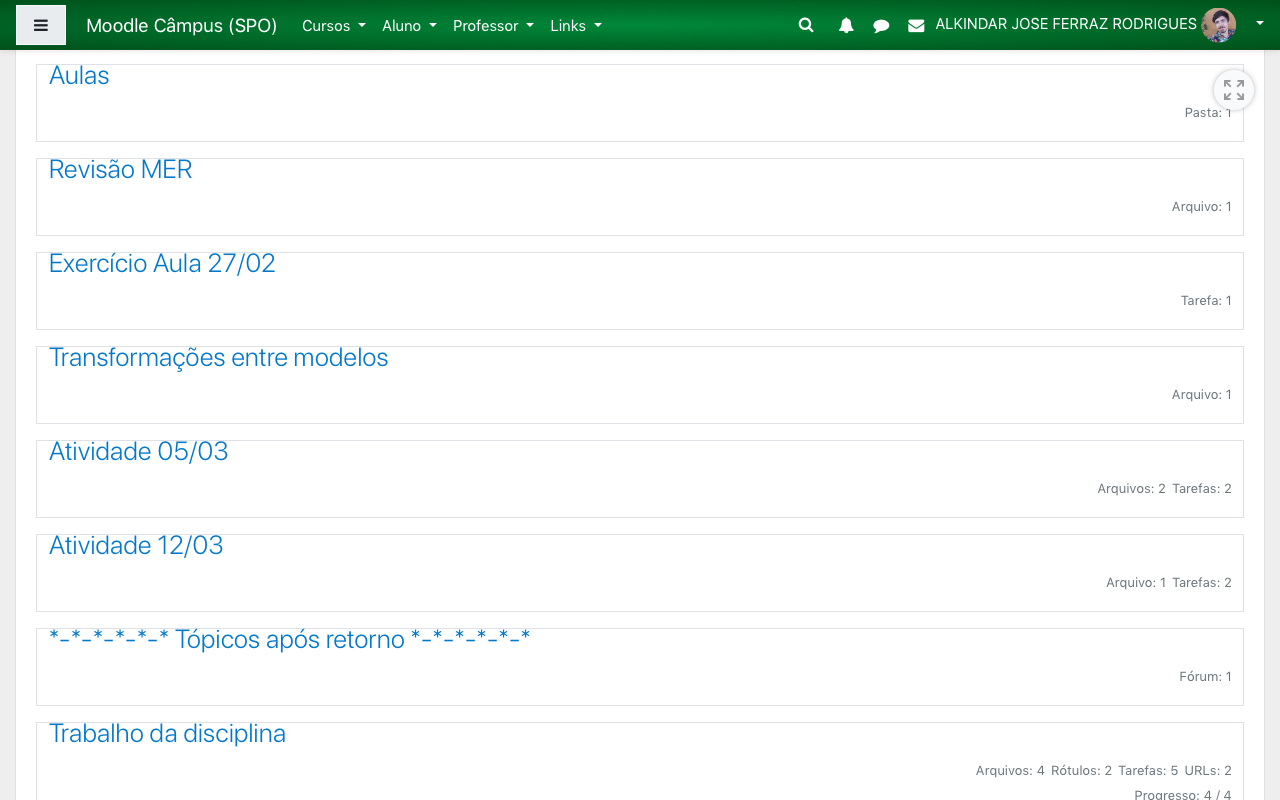
\includegraphics[width=.9\linewidth]{./media/disc_3.png}
\caption[\emph{Layout}]{\label{fig:org86fdd05}\emph{Layout} da página de disciplinas: tópicos em caixas largas, com detalhes sobre os materiais disponíveis a direita.}
\end{figure}
\end{document}
